
\documentclass[11pt,a4paper]{article}
\usepackage[T1]{fontenc}
\usepackage{lmodern}
\usepackage{amsmath,amssymb,amsfonts,mathtools}
\usepackage{graphicx,booktabs,longtable,array,tabularx,adjustbox}
\usepackage{geometry,microtype,fancyhdr,lastpage,etoolbox,enumitem}
\usepackage{newunicodechar,textcomp}
\usepackage{hyperref}
\hypersetup{hidelinks,pdfcreator={XeLaTeX / QM1 academic edition}}
\geometry{left=20mm,right=20mm,top=22mm,bottom=23mm}
\setcounter{secnumdepth}{2}
\setlength{\parindent}{0pt}
\setlength{\parskip}{4pt plus 1pt}
\setlength{\emergencystretch}{2em}
\setlength{\tabcolsep}{3pt}
\renewcommand{\arraystretch}{1.16}
\setlist{nosep,topsep=3pt,itemsep=2pt,leftmargin=7mm}
\AtBeginEnvironment{longtable}{\footnotesize\setlength{\tabcolsep}{2.2pt}}
\newcommand{\tightlist}{\setlength{\itemsep}{0pt}\setlength{\parskip}{0pt}}
\providecommand{\Cov}{\operatorname{Cov}}
\providecommand{\Var}{\operatorname{Var}}
\providecommand{\Corr}{\operatorname{Corr}}
\providecommand{\MAD}{\operatorname{MAD}}
\providecommand{\E}{\mathbb{E}}
\providecommand{\R}{\mathbb{R}}
\newunicodechar{—}{\textemdash}
\newunicodechar{–}{\textendash}
\newunicodechar{€}{\texteuro}
\newunicodechar{≤}{\ensuremath{\leq}}
\newunicodechar{≥}{\ensuremath{\geq}}
\newunicodechar{×}{\ensuremath{\times}}
\newunicodechar{÷}{\ensuremath{\div}}
\newunicodechar{Σ}{\ensuremath{\Sigma}}
\newunicodechar{σ}{\ensuremath{\sigma}}
\newunicodechar{μ}{\ensuremath{\mu}}
\newunicodechar{Δ}{\ensuremath{\Delta}}
\newunicodechar{∑}{\ensuremath{\sum}}
\newunicodechar{≈}{\ensuremath{\approx}}
\newunicodechar{√}{\ensuremath{\surd}}
\newunicodechar{≠}{\ensuremath{\ne}}
\newunicodechar{→}{\ensuremath{\to}}
\newunicodechar{∞}{\ensuremath{\infty}}
\newunicodechar{∈}{\ensuremath{\in}}
\newunicodechar{−}{\ensuremath{-}}
\newunicodechar{²}{\ensuremath{^{2}}}
\newunicodechar{³}{\ensuremath{^{3}}}
\newunicodechar{₀}{\ensuremath{_{0}}}
\newunicodechar{₁}{\ensuremath{_{1}}}
\newunicodechar{₂}{\ensuremath{_{2}}}
\newunicodechar{₃}{\ensuremath{_{3}}}
\newunicodechar{₄}{\ensuremath{_{4}}}
\newunicodechar{ₜ}{\ensuremath{_{t}}}
\newunicodechar{ₚ}{\ensuremath{_{p}}}
\newunicodechar{ₙ}{\ensuremath{_{n}}}
\newunicodechar{ₓ}{\ensuremath{_{x}}}
\newunicodechar{ᵢ}{\ensuremath{_{i}}}
\newunicodechar{ŷ}{\ensuremath{\hat y}}
\newunicodechar{Ŷ}{\ensuremath{\widehat Y}}
\newunicodechar{ₘ}{\ensuremath{_{m}}}
\newunicodechar{ₑ}{\ensuremath{_{e}}}
\newunicodechar{ₐ}{\ensuremath{_{a}}}
\newunicodechar{ₖ}{\ensuremath{_{k}}}
\newunicodechar{ₛ}{\ensuremath{_{s}}}
\newunicodechar{ₗ}{\ensuremath{_{l}}}
\newunicodechar{ₕ}{\ensuremath{_{h}}}
\newunicodechar{ₒ}{\ensuremath{_{o}}}
\newunicodechar{₊}{\ensuremath{_{+}}}
\newunicodechar{₋}{\ensuremath{_{-}}}
\newunicodechar{₌}{\ensuremath{_{=}}}
\newunicodechar{₍}{\ensuremath{_{(}}}
\newunicodechar{₎}{\ensuremath{_{)}}}
\newunicodechar{⁻}{\ensuremath{^{-}}}
\newunicodechar{⁺}{\ensuremath{^{+}}}
\newunicodechar{⁰}{\ensuremath{^{0}}}
\newunicodechar{¹}{\ensuremath{^{1}}}
\newunicodechar{⁴}{\ensuremath{^{4}}}
\newunicodechar{⁵}{\ensuremath{^{5}}}
\newunicodechar{⁶}{\ensuremath{^{6}}}
\newunicodechar{⁷}{\ensuremath{^{7}}}
\newunicodechar{⁸}{\ensuremath{^{8}}}
\newunicodechar{⁹}{\ensuremath{^{9}}}
\makeatletter
\renewcommand{\section}{\@startsection{section}{1}{0pt}{2.0ex plus .7ex minus .3ex}{1.0ex}{\large\bfseries}}
\renewcommand{\subsection}{\@startsection{subsection}{2}{0pt}{1.8ex plus .5ex minus .2ex}{.7ex}{\normalsize\bfseries}}
\renewcommand{\subsubsection}{\@startsection{subsubsection}{3}{0pt}{1.3ex plus .4ex minus .2ex}{.5ex}{\normalsize\bfseries}}
\makeatother
\pagestyle{fancy}
\fancyhf{}
\renewcommand{\headrulewidth}{0.35pt}
\renewcommand{\footrulewidth}{0pt}
\fancyhead[L]{\small\textsc{KEDGE Business School --- QM1}}
\fancyhead[R]{\small\textsc{2026--2027}}
\fancyfoot[L]{\small Badr ABOUFARASSE, PhD}
\fancyfoot[R]{\small\thepage\ /\ \pageref{LastPage}}
\setlength{\headheight}{14pt}
\setkeys{Gin}{keepaspectratio}
\begin{document}

\begin{center}
{\small\textsc{KEDGE Business School \quad EBP1 \quad Quantitative Methods 1}}\\[6pt]
{\Large\bfseries Worksheet 1 — Presenting and organising data}\\[6pt]
{\normalsize\bfseries Fully worked solutions}\\[6pt]
{\small Badr ABOUFARASSE, PhD \quad --- \quad 2026--2027}
\end{center}
\vspace{2mm}\hrule\vspace{6mm}

\hypertarget{core-applications}{%
\section{Core applications}\label{core-applications}}

Master the essential definitions and calculations from the course.

\emph{Core application --- 10 min}

\hypertarget{exercise-1-population-sample-and-variable-types}{%
\subsection{Exercise 1 -- Population, sample and variable types}\label{exercise-1-population-sample-and-variable-types}}

A store wants to study all customers who made a purchase in September. It surveys a sample of 80 customers and records:

\begin{longtable}[]{@{}p{0.32\linewidth}p{0.62\linewidth}@{}}
\toprule\noalign{}
Variable & Example \\
\midrule\noalign{}
\endhead
\bottomrule\noalign{}
\endlastfoot
Payment method & card, cash, mobile \\
Number of items purchased & 1, 2, 3, \ldots{} \\
Time spent in store & minutes \\
Satisfaction level & very dissatisfied to very satisfied \\
\end{longtable}

\begin{enumerate}
\item
  Identify the target population, the sample and the statistical unit.
\item
  Classify each variable as nominal qualitative, ordinal qualitative, discrete quantitative or continuous quantitative.
\item
  Choose an appropriate graph for each variable.
\item
  For which variables do cumulative frequencies make sense? Explain.
\item
  Explain why a large sample is not necessarily representative.
\end{enumerate}

\hypertarget{fully-worked-solution}{%
\subsubsection{Fully worked solution}\label{fully-worked-solution}}

Target population: all customers who made a purchase in September. Sample: the 80 surveyed customers. Statistical unit: one customer.

\begin{longtable}[]{@{}lll@{}}
\toprule\noalign{}
Variable & Type & Suitable graph \\
\midrule\noalign{}
\endhead
\bottomrule\noalign{}
\endlastfoot
Payment method & nominal qualitative & bar chart / pie chart \\
Number of items & discrete quantitative & stick/bar diagram \\
Time in store & continuous quantitative & histogram \\
Satisfaction & ordinal qualitative & ordered bars \\
\end{longtable}

Cumulative frequencies are meaningful for ordered variables: number of items, time and satisfaction. They are not meaningful for payment method because nominal categories have no natural order.

A large sample may still be biased if selection is not representative. For example, a voluntary survey may attract more highly satisfied or highly engaged customers.

\emph{Core application --- 20 min}

\hypertarget{exercise-2-discrete-distribution}{%
\subsection{Exercise 2 -- Discrete distribution}\label{exercise-2-discrete-distribution}}

\begin{longtable}[]{@{}lllllll@{}}
\toprule\noalign{}
{\(x_i\)} & 0 & 1 & 2 & 3 & 4 & 5 \\
\midrule\noalign{}
\endhead
\bottomrule\noalign{}
\endlastfoot
{\(n_i\)} & 3 & 7 & 12 & 10 & 6 & 2 \\
\end{longtable}

\begin{enumerate}
\item
  Check the total count {\(N\)}.
\item
  Calculate relative frequencies {\(f_i=n_i/N\)} and increasing cumulative frequencies.
\item
  Draw a stick/bar diagram.
\item
  Construct the cumulative distribution function {\(F(x)=P(X\leq x)\)}.
\item
  Find the proportion of customers who placed at most three orders.
\end{enumerate}

\hypertarget{fully-worked-solution-1}{%
\subsubsection{Fully worked solution}\label{fully-worked-solution-1}}

{\[N=3+7+12+10+6+2=40.\]}

\begin{longtable}[]{@{}lllllll@{}}
\toprule\noalign{}
{\(x_i\)} & 0 & 1 & 2 & 3 & 4 & 5 \\
\midrule\noalign{}
\endhead
\bottomrule\noalign{}
\endlastfoot
{\(n_i\)} & 3 & 7 & 12 & 10 & 6 & 2 \\
{\(f_i\)} & 0.075 & 0.175 & 0.300 & 0.250 & 0.150 & 0.050 \\
{\(F_i\)} & 0.075 & 0.250 & 0.550 & 0.800 & 0.950 & 1.000 \\
\end{longtable}

For example: {\[f_2=\frac{12}{40}=0.30=30\%.\]} The proportion with at most three orders is: {\[F(3)=\frac{3+7+12+10}{40}=\frac{32}{40}=0.80=80\%.\]}

Charts from the counts: the cumulative distribution reaches 80\% at x=3.

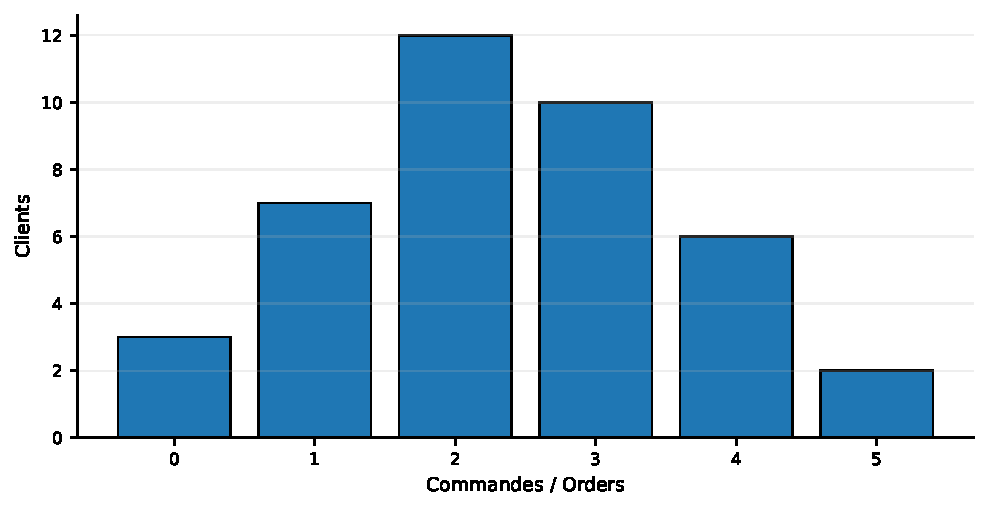
\includegraphics[width=0.82\textwidth,height=\textheight]{assets/chapter-1-solutions-en-datachart-01.pdf}

\emph{Nombre de commandes / Orders}

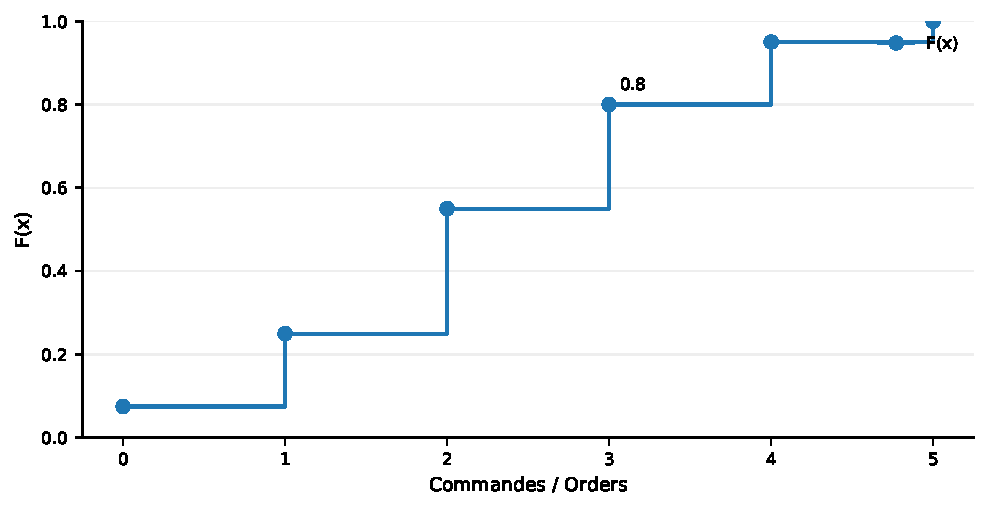
\includegraphics[width=0.82\textwidth,height=\textheight]{assets/chapter-1-solutions-en-datachart-02.pdf}

\emph{Fonction de répartition / Empirical CDF}

\hypertarget{complete-cumulative-table}{%
\subsubsection{Complete cumulative table}\label{complete-cumulative-table}}

\begin{longtable}[]{@{}lllllll@{}}
\toprule\noalign{}
x & n & f=n/40 & ECC & ECD & FCC & FCD \\
\midrule\noalign{}
\endhead
\bottomrule\noalign{}
\endlastfoot
0 & 3 & 3/40=.075 & 3 & 40 & .075 & 1.000 \\
1 & 7 & 7/40=.175 & 10 & 37 & .250 & .925 \\
2 & 12 & 12/40=.300 & 22 & 30 & .550 & .750 \\
3 & 10 & 10/40=.250 & 32 & 18 & .800 & .450 \\
4 & 6 & 6/40=.150 & 38 & 8 & .950 & .200 \\
5 & 2 & 2/40=.050 & 40 & 2 & 1.000 & .050 \\
\end{longtable}

At x=3, ascending count=3+7+12+10=32 and descending count=10+6+2=18. Ascending cumulative frequencies measure P(X≤x), descending ones P(X≥x).

\emph{Core application --- 15 min}

\hypertarget{extra-1-cross-tabulation-and-conditional-percentages}{%
\subsection{Extra 1 --- Cross-tabulation and conditional percentages}\label{extra-1-cross-tabulation-and-conditional-percentages}}

Among 120 students, 50 use public transport, including 30 women. Of the 70 other students, 35 are women.

\begin{enumerate}
\tightlist
\item
  Build the gender × transport table.
\item
  Compute the public-transport rate within each gender.
\item
  State whether an association appears present.
\end{enumerate}

\textbf{Method hint:}

Conditional percentages use the total of the conditioning group as denominator.

\hypertarget{fully-worked-solution-2}{%
\subsubsection{Fully worked solution}\label{fully-worked-solution-2}}

The table is: women 30 public and 35 other; men 20 public and 35 other. Totals are 65 women and 55 men. Conditional rates are 30/65 = 46.2\% for women and 20/55 = 36.4\% for men.

The sample shows a 9.8-point difference. This is descriptive evidence of association, not proof of a population difference or causal effect.

\hypertarget{assessment-and-exam-practice}{%
\section{Assessment and exam practice}\label{assessment-and-exam-practice}}

Practise independently with assessment and final-exam style questions.

\emph{Assessment / exam practice --- 40 min}

\hypertarget{exercise-3-continuous-variable-with-unequal-class-widths}{%
\subsection{Exercise 3 -- Continuous variable with unequal class widths}\label{exercise-3-continuous-variable-with-unequal-class-widths}}

\begin{longtable}[]{@{}llllllllll@{}}
\toprule\noalign{}
Class & {\([10,14[\)} & {\([14,18[\)} & {\([18,26[\)} & {\([26,30[\)} & {\([30,35[\)} & {\([35,40[\)} & {\([40,45[\)} & {\([45,50[\)} & {\([50,55[\)} \\
\midrule\noalign{}
\endhead
\bottomrule\noalign{}
\endlastfoot
{\(n_i\)} & 4 & 12 & 32 & 32 & 60 & 35 & 25 & 5 & 5 \\
\end{longtable}

\begin{enumerate}
\item
  For each class, calculate width {\(a_i\)}, relative frequency {\(f_i\)} and count density {\(d_i=n_i/a_i\)}.
\item
  Draw the correct histogram and explain why raw counts cannot be used as heights when class widths differ.
\item
  Calculate increasing and decreasing cumulative counts and the corresponding cumulative relative frequencies.
\item
  Draw the cumulative curves.
\item
  Find the number and proportion willing to pay less than 35 euros, then at least 35 euros.
\end{enumerate}

\hypertarget{fully-worked-solution-3}{%
\subsubsection{Fully worked solution}\label{fully-worked-solution-3}}

\begin{longtable}[]{@{}llllllllll@{}}
\toprule\noalign{}
Class & {\([10,14[\)} & {\([14,18[\)} & {\([18,26[\)} & {\([26,30[\)} & {\([30,35[\)} & {\([35,40[\)} & {\([40,45[\)} & {\([45,50[\)} & {\([50,55[\)} \\
\midrule\noalign{}
\endhead
\bottomrule\noalign{}
\endlastfoot
{\(n_i\)} & 4 & 12 & 32 & 32 & 60 & 35 & 25 & 5 & 5 \\
{\(a_i\)} & 4 & 4 & 8 & 4 & 5 & 5 & 5 & 5 & 5 \\
{\(f_i(\%)\)} & 1.90 & 5.71 & 15.24 & 15.24 & 28.57 & 16.67 & 11.90 & 2.38 & 2.38 \\
{\(d_i\)} & 1 & 3 & 4 & 8 & 12 & 7 & 5 & 1 & 1 \\
ICC & 4 & 16 & 48 & 80 & 140 & 175 & 200 & 205 & 210 \\
DCC & 210 & 206 & 194 & 162 & 130 & 70 & 35 & 10 & 5 \\
\end{longtable}

For example: {\[f_{[18,26[}=\frac{32}{210}\approx0.1524=15.24\%,
\qquad d_{[18,26[}=\frac{32}{8}=4.\]} With unequal class widths, rectangle area must represent the count, so density is used as height.

Less than 35 euros: {\[140,\qquad
\frac{140}{210}=66.67\%.\]} At least 35 euros: {\[70,\qquad \frac{70}{210}=33.33\%.\]}

Complete table: fᵢ=nᵢ/210; cumulative relative frequencies are ECC/210 and ECD/210. Cumulative plots use class boundaries.

\begin{longtable}[]{@{}lllllllll@{}}
\toprule\noalign{}
Classe & aᵢ & nᵢ & fᵢ (\%) & dᵢ & ECC & ECD & FCC (\%) & FCD (\%) \\
\midrule\noalign{}
\endhead
\bottomrule\noalign{}
\endlastfoot
{[}10,14{[} & 4 & 4 & 1.90 & 1 & 4 & 210 & 1.90 & 100.00 \\
{[}14,18{[} & 4 & 12 & 5.71 & 3 & 16 & 206 & 7.62 & 98.10 \\
{[}18,26{[} & 8 & 32 & 15.24 & 4 & 48 & 194 & 22.86 & 92.38 \\
{[}26,30{[} & 4 & 32 & 15.24 & 8 & 80 & 162 & 38.10 & 77.14 \\
{[}30,35{[} & 5 & 60 & 28.57 & 12 & 140 & 130 & 66.67 & 61.90 \\
{[}35,40{[} & 5 & 35 & 16.67 & 7 & 175 & 70 & 83.33 & 33.33 \\
{[}40,45{[} & 5 & 25 & 11.90 & 5 & 200 & 35 & 95.24 & 16.67 \\
{[}45,50{[} & 5 & 5 & 2.38 & 1 & 205 & 10 & 97.62 & 4.76 \\
{[}50,55{[} & 5 & 5 & 2.38 & 1 & 210 & 5 & 100.00 & 2.38 \\
TOTAL & --- & 210 & 100 & --- & 210 & --- & 100 & --- \\
\end{longtable}

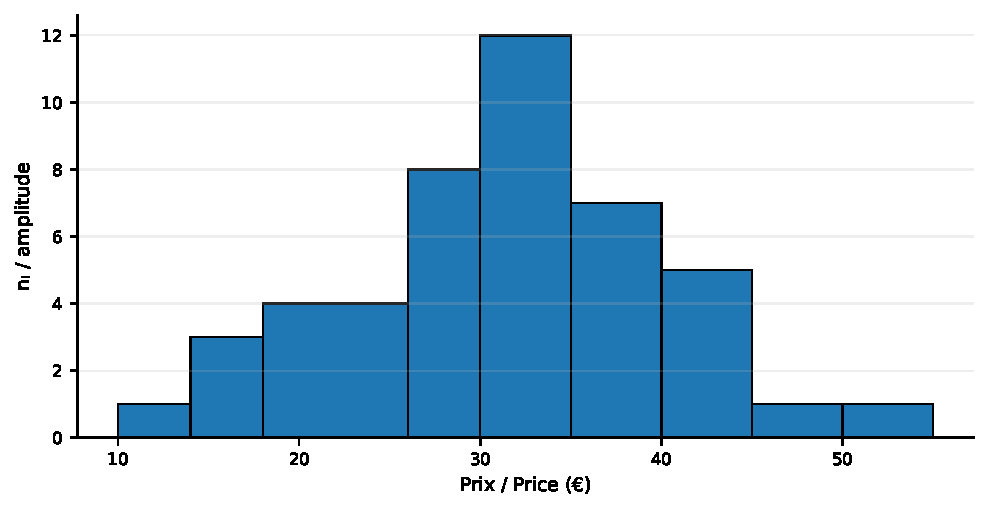
\includegraphics[width=0.82\textwidth,height=\textheight]{assets/chapter-1-solutions-en-datachart-03.pdf}

\emph{Histogramme des densités / Density histogram}

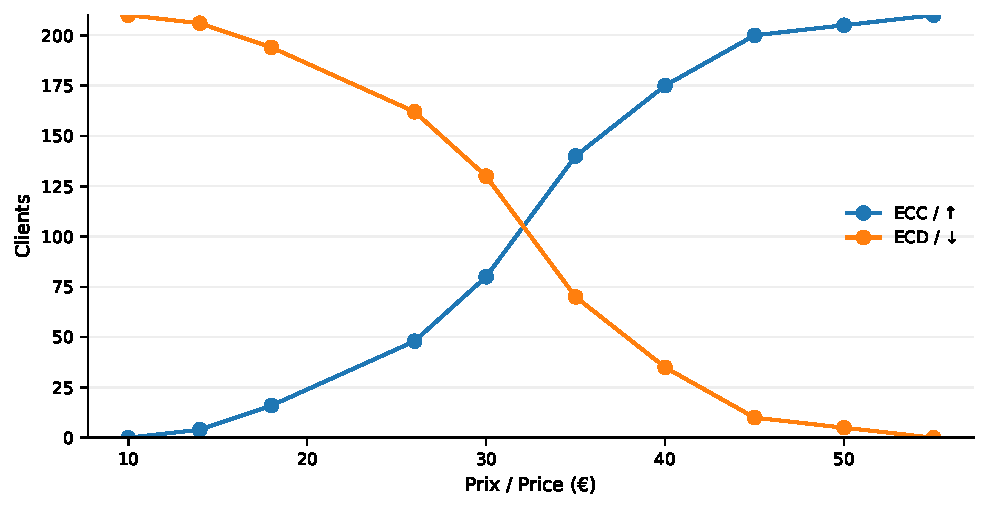
\includegraphics[width=0.82\textwidth,height=\textheight]{assets/chapter-1-solutions-en-datachart-04.pdf}

\emph{Effectifs cumulés / Cumulative counts}

\emph{Assessment / exam practice --- 35 min}

\hypertarget{extra-3-continuous-assessment-case-willingness-to-pay}{%
\subsection{Extra 3 --- Continuous-assessment case: willingness to pay}\label{extra-3-continuous-assessment-case-willingness-to-pay}}

\textbf{Case study --- 12 marks.} A food retailer asks 200 customers for the maximum price they would pay for a sustainable lunch box.

\begin{longtable}[]{@{}lllllll@{}}
\toprule\noalign{}
Maximum price (€) & {[}20,25{[} & {[}25,30{[} & {[}30,40{[} & {[}40,50{[} & {[}50,60{[} & {[}60,80{[} \\
\midrule\noalign{}
\endhead
\bottomrule\noalign{}
\endlastfoot
Customers & 10 & 20 & 50 & 60 & 40 & 20 \\
\end{longtable}

\begin{enumerate}
\tightlist
\item
  Identify the population, statistical unit, variable and variable type. \emph{(2 marks)}
\item
  Calculate class widths, relative frequencies and frequency densities. \emph{(3 marks)}
\item
  Explain how to construct the correct histogram and identify the modal class. \emph{(2 marks)}
\item
  Calculate ascending and descending cumulative counts. Give the coordinates needed to draw both cumulative curves. \emph{(3 marks)}
\item
  Find the highest price that at least 60\% of surveyed customers would be willing to pay. Explain the percentile used. \emph{(2 marks)}
\end{enumerate}

\textbf{Method hint:}

Unequal-width classes require frequency density. For the pricing decision, translate ``at least 60\% can pay'' into an ascending cumulative percentage.

\hypertarget{fully-worked-solution-4}{%
\subsubsection{Fully worked solution}\label{fully-worked-solution-4}}

\hypertarget{detailed-solution-and-marking-logic}{%
\subsubsection{Detailed solution and marking logic}\label{detailed-solution-and-marking-logic}}

\textbf{1.} Population: the 200 surveyed customers; unit: one surveyed customer; variable: maximum willingness to pay in euros; type: quantitative continuous.

\begin{longtable}[]{@{}llllll@{}}
\toprule\noalign{}
Class & Width & Count & Frequency & Density (count/width) & Ascending count \\
\midrule\noalign{}
\endhead
\bottomrule\noalign{}
\endlastfoot
{[}20,25{[} & 5 & 10 & 5\% & 2 & 10 \\
{[}25,30{[} & 5 & 20 & 10\% & 4 & 30 \\
{[}30,40{[} & 10 & 50 & 25\% & 5 & 80 \\
{[}40,50{[} & 10 & 60 & 30\% & 6 & 140 \\
{[}50,60{[} & 10 & 40 & 20\% & 4 & 180 \\
{[}60,80{[} & 20 & 20 & 10\% & 1 & 200 \\
\end{longtable}

\textbf{2--3.} Because widths differ, histogram heights must be densities, not raw counts. The largest density is 6, so the modal class is {[}40,50{[}.

\textbf{4.} The ascending curve passes through (20,0), (25,10), (30,30), (40,80), (50,140), (60,180), (80,200). The descending curve uses (20,200), (25,190), (30,170), (40,120), (50,60), (60,20), (80,0).

\textbf{5.} If at least 60\% must be able to pay, no more than 40\% may have a willingness to pay below the chosen price. Forty per cent of 200 is 80, reached at €40. The decision uses the 40th percentile, not the 60th: the recommended maximum price is therefore \textbf{€40}.

\textbf{Exam habit.} State the rule, show the calculation, then interpret the result in the context of the decision.

Full table and charts (histogram heights = counts/class widths):

\begin{longtable}[]{@{}lllllllll@{}}
\toprule\noalign{}
Classe / Class & nᵢ & aᵢ & fᵢ (\%) & dᵢ & ECC & ECD & FCC (\%) & FCD (\%) \\
\midrule\noalign{}
\endhead
\bottomrule\noalign{}
\endlastfoot
{[}20,25{[} & 10 & 5 & 5.00 & 2 & 10 & 200 & 5.00 & 100.00 \\
{[}25,30{[} & 20 & 5 & 10.00 & 4 & 30 & 190 & 15.00 & 95.00 \\
{[}30,40{[} & 50 & 10 & 25.00 & 5 & 80 & 170 & 40.00 & 85.00 \\
{[}40,50{[} & 60 & 10 & 30.00 & 6 & 140 & 120 & 70.00 & 60.00 \\
{[}50,60{[} & 40 & 10 & 20.00 & 4 & 180 & 60 & 90.00 & 30.00 \\
{[}60,80{[} & 20 & 20 & 10.00 & 1 & 200 & 20 & 100.00 & 10.00 \\
\end{longtable}

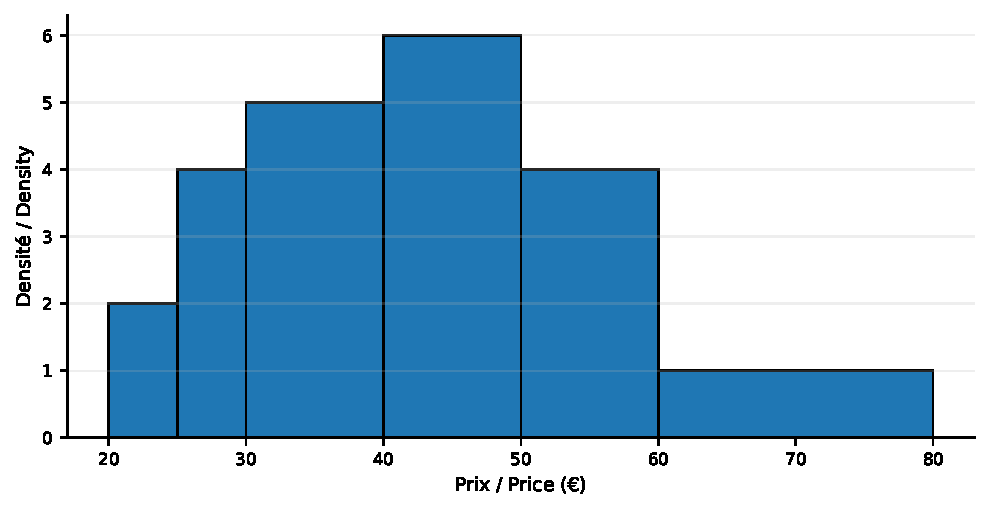
\includegraphics[width=0.82\textwidth,height=\textheight]{assets/chapter-1-solutions-en-datachart-05.pdf}

\emph{Consentement à payer / Willingness-to-pay histogram}

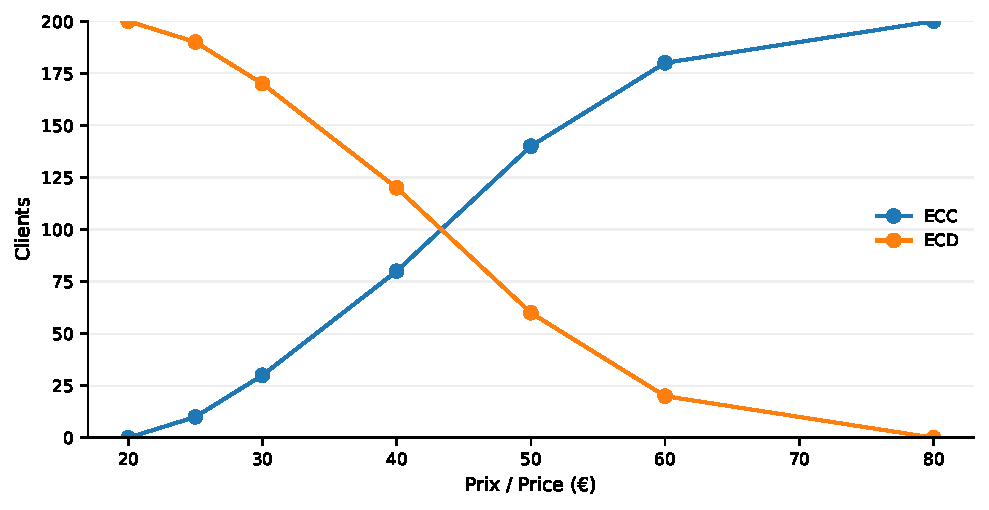
\includegraphics[width=0.82\textwidth,height=\textheight]{assets/chapter-1-solutions-en-datachart-06.pdf}

\emph{Courbes cumulatives / Cumulative counts}

The €40 threshold is the 40th percentile: 80 out of 200 customers accept less than €40, so approximately 60\% can afford at least €40.

\emph{Assessment / exam practice --- 30 min}

\hypertarget{extra-4-exam-style-synthesis-reporting-customer-satisfaction}{%
\subsection{Extra 4 --- Exam-style synthesis: reporting customer satisfaction}\label{extra-4-exam-style-synthesis-reporting-customer-satisfaction}}

\textbf{Independent case --- 10 marks.} Two stores collect satisfaction ratings on an ordered scale from 1 (very dissatisfied) to 5 (very satisfied).

\begin{longtable}[]{@{}lllllll@{}}
\toprule\noalign{}
Rating & 1 & 2 & 3 & 4 & 5 & Total \\
\midrule\noalign{}
\endhead
\bottomrule\noalign{}
\endlastfoot
Store A & 6 & 10 & 18 & 36 & 30 & 100 \\
Store B & 4 & 12 & 30 & 34 & 20 & 100 \\
\end{longtable}

\begin{enumerate}
\tightlist
\item
  Identify the variable and its measurement scale. \emph{(1 mark)}
\item
  Choose and justify one graph for comparing the two stores. Describe precisely how it should be constructed. \emph{(2 marks)}
\item
  Compute, for each store, the percentages rated 4 or 5 and the cumulative percentage rated at most 2. \emph{(3 marks)}
\item
  A manager says: ``Store A is 50\% better because it has 30 ratings of 5 versus 20.'' Criticise this claim. \emph{(2 marks)}
\item
  Write a three-sentence statistical conclusion, including one limitation of the survey. \emph{(2 marks)}
\end{enumerate}

\textbf{Method hint:}

Keep the order of the categories, compare percentages because the store totals could differ in another dataset, and separate description from causation.

\hypertarget{fully-worked-solution-5}{%
\subsubsection{Fully worked solution}\label{fully-worked-solution-5}}

\textbf{1.} Satisfaction is qualitative ordinal: categories have a meaningful order, but the distances between adjacent ratings are not guaranteed equal.

\textbf{2.} Use grouped bars or a 100\% stacked ordered bar chart. Keep ratings 1--5 in order, use identical axes and colours, and show percentages. A histogram is inappropriate because the categories are ordinal, not continuous intervals.

\textbf{3.} Store A: ratings 4--5 = (36+30)/100 = \textbf{66\%}; ratings at most 2 = (6+10)/100 = \textbf{16\%}. Store B: ratings 4--5 = (34+20)/100 = \textbf{54\%}; ratings at most 2 = (4+12)/100 = \textbf{16\%}.

\textbf{4.} Thirty is indeed 50\% greater than twenty, but this isolates one category and does not mean that the store is ``50\% better''. Across ratings 4--5, the difference is 12 percentage points; the sampling method and uncertainty are unknown, and no causal conclusion follows.

\textbf{5. Model conclusion.} ``In the surveyed samples, Store A has a higher share of favourable ratings (66\%) than Store B (54\%), while both have 16\% ratings of 1 or 2. The difference is descriptive and does not by itself establish that Store A provides better service. Before generalising, we need to know how customers were selected, the response rates and whether the survey periods were comparable.''

\hypertarget{optional-advanced-practice}{%
\section{Optional advanced practice}\label{optional-advanced-practice}}

Explore additional interpretations and professional applications.

\emph{Advanced practice --- 15 min}

\hypertarget{extra-2-data-quality-and-communication-protocol}{%
\subsection{Extra 2 --- Data-quality and communication protocol}\label{extra-2-data-quality-and-communication-protocol}}

A CRM extract contains duplicate customers, missing ages coded 999, inconsistent dates and revenue recorded in euros and thousands of euros. Propose a reproducible six-step protocol before producing a management dashboard.

\textbf{Method hint:}

Separate validation, cleaning, documentation and communication.

\hypertarget{fully-worked-solution-6}{%
\subsubsection{Fully worked solution}\label{fully-worked-solution-6}}

\begin{enumerate}
\tightlist
\item
  Preserve an immutable raw file and identifiers.
\item
  Define a data dictionary and units.
\item
  Detect duplicates and specify a defensible retention rule.
\item
  Recode 999 as missing and report missingness by group.
\item
  Validate dates, ranges and logical consistency.
\item
  Standardise monetary units, document every transformation and publish checks with the dashboard.
\end{enumerate}

Never silently replace missing observations or delete unusual values.

\end{document}
